\documentclass[12pt, titlepage]{article}

\usepackage{amsmath}
\usepackage[margin = 1in]{geometry}
\usepackage{graphicx}
\usepackage{booktabs}
\usepackage{natbib}
\usepackage{array}

\usepackage{lipsum}
\usepackage[colorlinks=true, citecolor=blue]{hyperref}


%% meta data

\title{Proposal: Association between Breast Cancer and Hepatitis C Virus}
\author{Amy Traianou\\
  Department of Statistics\\
  University of Connecticut
}

\begin{document}
\maketitle


\paragraph{Introduction}

For this paper I decided to explore the risk factors associated with breast cancer in women. Breast cancer is extremely
prevalent and researchers are constantly trying to determine risk factors to identify women for preventative exams.
There are many studies attempting to determine if there is an association between certain risk factors and 
breast cancer including chronic hepatitis C infection \citep{Larrey2010is} and hepatitis B \citep{vishnu2016does}. 


\paragraph{Specific Aims}
Specifically, I want to determine if there is an association between testing positive for hepatitis C virus
and breast cancer. Both Hepatitis C and breast cancer are extremely prevalent in Egypt \citep{Hussein2021high}. 
Very recently on October 6th, Egypt and Qatar agreed to collaborate in the health sector and use each 
other's expertise. The health ministers specifically mentioned research in Hepatitis C and breast cancer
as a area of interest \citep{arham2022egypt}. Thus, research surrounding these diseases is becoming more
important in the field. 

\paragraph{Data}

The data I will be using is from a retrospective case control study conducted in 2020 \citep{2020association}. The data includes 405 subjects as
part of the study group, all having been treated for breast cancer in the past 10 years. The second group consists of 145 adult females
from a governorate in Egypt, who all participated in a cross-sectional study from 2015-2017. This data can be put into a 2x2 contingency table
for statistical analysis. 

\begin{tabular}{ | m{5cm} | m{3cm}| m{3cm} | m{2cm} | }
  \hline
  Risk Factor & Study Group & Control & Total\\ 
  \hline
  Anti-HCV Seropositive & 88 & 15 & 103 \\ 
  \hline
  Anti-HCV Seronegative & 317 & 130 & 447 \\ 
  \hline
  Total & 405 & 145 & 550 \\ 
  \hline
\end{tabular}


\paragraph{Research Design and Methods}

To test the association of breast cancer and Hepatitis C, I am going to use either the chi-square or Fisher's Exact test, depending on the
conditions from the sample size \citep{warner2013testing}. Fisher's exact test is useful for when the normality assumption is violated 
and the expected values of the 2x2 table are too small. The test uses the hypergeometric distribution to test if the probabilities are
the same between the two groups. Thus, we can determine if there is more of a risk of breast cancer for those with seropositive Hep C. As
 a result, we can determine if women who chronically test positive should be tested more frequently because they are at a higher risk. 
 
Figure~\ref{fig:formula} shows the probability of the original table occuring.

\begin{figure}[tbp]
  \centering
  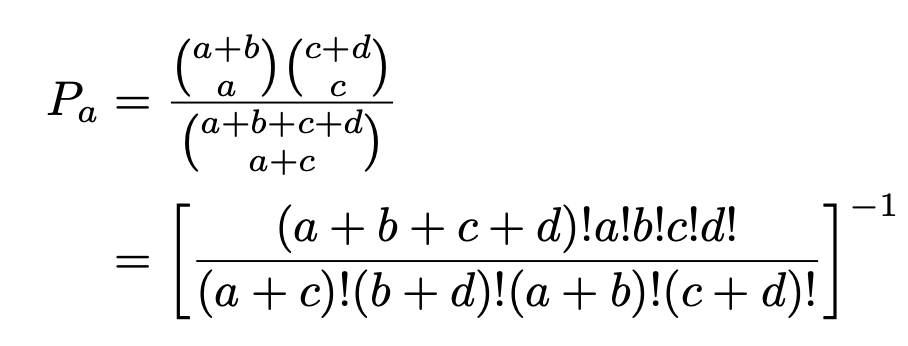
\includegraphics[width=8cm]{formula.png}
  \caption{This is the hypergeometric pmf.}
  \label{fig:formula}
\end{figure}


\paragraph{Discussion}

I expect to find an association between hepatitis C and breast cancer because there is some existing research that agrees with the association.
Therefore, this paper would corroborate the exisitng assumptions while giving them more of a basis. Although the potential impacts are quite 
minimal, the more research that supports the association, the better. If the investigation is not what I expect, then I would suggest more
data needs to be collected surrounding women with breast cancer in Eygpt. Specifically, a full prospective study with new samples. 

\paragraph{Conclusion}

In conclusion, I propose using data from women in Egypt to determine if there is an association between seropositive Hepatitis C and 
breast cancer. The Egyptian government has identified breast cancer as an area of interest for medical research so it has importance in
the field. Additionally, identifying a new risk factor for breast cancer would increase preventative screening in adult women and hopefully 
improve the ability to discover cancer in earlier stages. 



\bibliography{.../manuscript/refs.bibliography}
\bibliographystyle{chicago}

\end{document}